\documentclass[12pt,twoside]{report}

% PACCHETTI FONDAMENTALI
\usepackage{amsmath,amsfonts,amssymb,amsthm, dsfont, mathtools}
\usepackage{graphicx}
\usepackage[a4paper,outer=2cm,inner=3cm,top=3.3cm,bottom=2.5cm]{geometry}
\usepackage{float} % per il comando [H] per le tabelle
\usepackage{enumerate} % per scegliere i caratteri degli elechi
\usepackage{accents}
\usepackage{esint}
% intestazione pagine
\usepackage{fancyhdr}
% disegni
\usepackage{pgfplots}

% NOMENCLATURA
% indice
\renewcommand*\contentsname{Indice}
% capitoli
\renewcommand{\chaptername}{Capitolo}
% appendici
\renewcommand{\appendixname}{Appendice}
% bibliografia
\renewcommand\bibname{Bibliografia}

% TITOLI
% per mettere i titoli dei capitoli sulla destra e aggiungere una riga di separazione sotto
\usepackage{titlesec} 
\newcommand*{\justifyheading}{\raggedleft}
\titleformat{\chapter}[display]
  {\normalfont\LARGE\bfseries\justifyheading}
  {\chaptertitlename\ \thechapter \vspace*{-0.5cm}}
  {20pt}{\Huge}
  [\vspace*{0.3cm}\hrule height 0.08cm \vspace*{1cm}]

% STUTTURE FONDAMENTALI
% teoremi
\theoremstyle{plain}
\newtheorem{theorem}{Teorema}[section]
% lemmi
\newtheorem{lemma}[theorem]{Lemma}
% teoremi con nomi
\newtheoremstyle{named}{}{}{\itshape}{}{\bfseries}{.}{.5em}{\thmnote{#3} #2}
\theoremstyle{named}
\newtheorem{namedtheorem}[theorem]{Teorema}
% ipotesi
\newenvironment{ipotesi}%
{\quad\left|\quad\def\arraystretch{1.2}\begin{array}{@{}l@{}}}%
{\end{array}\right.}
% tesi
\newcommand{\tesi}[1]{\quad\left|\quad{#1}\right.}
% unico comando per ipotesi e tesi
\newcommand{\hpth}[2]
{
\begin{flalign*}
\quad\quad
\text{Ipotesi}
&\begin{ipotesi}
#1
\end{ipotesi}&&\\
\quad\quad
\text{Tesi}
&\tesi{#2}&&
\end{flalign*}
}
% più righe nella tesi 
\newcommand{\hpthml}[2]
{
\begin{flalign*}
\quad\quad
\text{Ipotesi}
&\begin{ipotesi}
#1
\end{ipotesi}&&\\
\quad\quad
\text{Tesi}
&\begin{ipotesi}
#2
\end{ipotesi}&&
\end{flalign*}
}
% quando ci sono 2 tesi distinte
\newcommand{\hpthth}[3]
{
\begin{flalign*}
\quad\quad
\text{Ipotesi}
&\begin{ipotesi} 
#1
\end{ipotesi}&&\\
\quad\quad
\text{Tesi 1}
&\tesi{#2}&&\\
\quad\quad
\text{Tesi 2}
&\tesi{#3}&&
\end{flalign*}
}
% dimostrazioni
\renewcommand*{\proofname}{\bf{Dimostrazione:}}
\renewcommand\qedsymbol{\textsc{qed}}
% definizioni
\theoremstyle{definition}
\newtheorem{definition}{Definzione}[section]
% esempi
\newtheorem{example}{Esempio}
% osservazioni
\theoremstyle{remark}
\newtheorem*{remark}{Osservazione}

% NOTAZIONE
% sistemi
\newenvironment{system}%
{\left\lbrace\begin{array}{@{}l@{}}}%
{\end{array}\right.}
% parte intera
\newcommand{\interior}[1]{\accentset{\circ}{#1}}
% norma
\newcommand\norm[1]{\left\lVert#1\right\rVert}
% absolute value
\newcommand\abs[1]{\left|#1\right|}

% PAGINA BIANCA
\usepackage{afterpage}
\newcommand\blankpage{%
    \null
    \thispagestyle{empty}%
    \newpage}

% ALTRI
% indentazione del testo a 0
\parindent 0px
% numerazione in align*
\newcommand\numberthis{\addtocounter{equation}{1}\tag{\theequation}}
% citazione
\usepackage{epigraph}
% immagini
\usepackage{wrapfig}
\usepackage[labelformat=empty]{caption}
% avoid hyphenation 
\emergencystretch=\maxdimen
\hyphenpenalty=10000
\hbadness=10000
% matrici
\makeatletter
\renewcommand*\env@matrix[1][*\c@MaxMatrixCols c]{%
  \hskip -\arraycolsep
  \let\@ifnextchar\new@ifnextchar
  \array{#1}}
\makeatother




\begin{document}

% non contare la pagina del titolo
\pagenumbering{gobble}

% titolo
\thispagestyle{empty}

\vspace*{-2.5cm} 
\mdseries{

\begin{center}
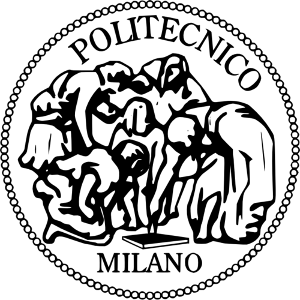
\includegraphics[width=5cm]{logo.png}

\vspace*{0.6cm}
{\Large\textsc{Politecnico di Milano}}\\
\rule{7cm}{1pt}

\vspace*{0.5cm}

Corso di Laurea Triennale in \textsc{Ingegneria Matematica}\\
Scuola di \textsc{Ingegneria Industriale e dell'Informazione}\\
\vspace*{1.3cm} 
{\LARGE\textmd{\textbf{
Sull'esistenza di soluzioni locali\\di equazioni differenziali\\\vspace*{0.2cm} alle derivate parziali
}}}

\vspace*{1.5truecm} 

{\small Tesi di}
{\large\vspace*{0.3cm}\\Alessandro Pedone}

\vspace*{1.3cm}

\begin{tabular}{@{}ll}
\small
Relatore:\\[0.5cm]
\normalsize
\quad Prof. Maurizio Grasselli & .......................................\\[1cm]
\small
Candidato:\\[0.5cm]
\normalsize
\quad Alessandro Pedone & .......................................\\
\end{tabular}
\vfill
\rule{6cm}{1pt}

\small
Sessione di Laurea Settembre 2024\\
Anno Accademico 2023/2024
\end{center} 
\clearpage
}
\blankpage

% conta con i numeri romani 
\pagenumbering{roman}

% citazione
\setlength\epigraphwidth{8cm}
\setlength\epigraphrule{0pt}
\vspace*{\fill}
\epigraph{\textit{All his life -- he had difficulty saying this, as he admitted, being always wary of too much enthusiasm -- all his life he had been waiting for such a student to come into this room. A student who would challenge him completely, who was not only capable of following the strivings of his own mind but perhaps of flying beyond them.}}{--- \textup{Alice Munro}, \textit{Too Much Happiness}}
\vspace*{\fill}
%indice
\tableofcontents

\newpage
\blankpage
\chapter*{Abstract}
\addcontentsline{toc}{chapter}{Abstract}

Sofya Kowalevski, la prima donna ad conseguire un dottorato in matematica in Europa, nel 1874 dava la luce alla dimostrazione del teorema di Cauchy-Kowalevski (TCK), il primo risultato generale per l'esistenza di soluzioni locali analitiche per equazioni differenziali alle derivate parziali (EDP) con dati di Cauchy.

\vspace{6mm}
La tesi mira a presentare questa pietra miliare della matematica esaltandone la profondità del dettaglio, le conseguenze e anche la semplicità delle idee che ha permesso di far emergere. A questo scopo sono ricorrenti i richiami di nozioni e risultati fondamentali ad affrontare il discorso e, inoltre, vengono trattate tutte le forme principali in cui è possibile enunciare il TCK.

\vspace{6mm}
A completamento sono presenti anche una sezione dedicata a tre esempi storicamente cruciali alla comprensione delle EDP e un'altra dedicata, invece, alle due sue fondamentali applicazioni: il teorema di Holmgren e il teorema di Cartan-Kähler.

\vspace{6mm}
\textbf{Parole chiave:} EDP, caratteristiche, analiticità/olomorfia, serie di potenze, metodo dei maggioranti, teoremi di Cauchy-Kowalevski, Holmgren e Cartan-Kähler

\newpage
\blankpage
%indice
\tableofcontents

% ricomincia a contare con i numeri arabi
\newpage
\blankpage
\pagenumbering{arabic}

% rimuovi i numeri a piè di pagina
\makeatletter
\let\ps@plain\ps@empty
\makeatother

% inserisci le intestazioni per i capitoli
\pagestyle{fancy}
\renewcommand{\chaptermark}[1]{\markboth{\textit{\thechapter.\ #1}}{}}
\renewcommand{\sectionmark}[1]{\markright{\textit{\thesection.\ #1}}}
\fancyhead{} % cancella tutti i campi
\fancyhead[RO,LE]{\bfseries \thepage}
\renewcommand{\headrulewidth}{0.4pt}
\cfoot{}
\fancyhead[LO]{\rightmark}
\fancyhead[RE]{\leftmark}
\setlength{\headheight}{18pt}

\chapter{Introduzione.}
Abbreviato CK

\section{Chi era Kowalevski?}

Sofya Vasilyevna Kovalevskaya

\textbf{Perché non Kovalevskaya}:  La stessa Kovalevskaya, per le pubblicazioni accademiche internazionali, soleva firmarsi Sophie Kowalevski

\textbf{Biografia}: background familiare, studi in germania, aiuto di Weierstrass (lezioni private e quattro tesi di dottorato), idee politiche (socialiste e radicali, sua sorella Anna le diede copies of radical journals of the time discussing Russian nihilism) e movimenti femministi, successo grazie alle tesi (I suoi risultati, tra cui il Teorema di Cauchy-Kovalevskaya, furono pubblicati nel 1875. Fu così che ottenne, prima donna in Europa, un dottorato in matematica), ritorno in russia inutile per la sua carriera accademica, in svezia dopo la morte del marito (Divenne, prima donna al mondo, professoressa di matematica, ottenendo la cattedra all'Università di Stoccolma (Högskola)), anche produzione letteraria, morte prematura a 41 anni nel 1891 di polmonite

\textbf{Nichilismo antico}: For the nihilists, science appeared to be the most effective means of helping the mass of people to a better life. Science pushed back the barriers of religion and superstition, and "proved" through the theory of evolution that (peaceful) social revolutions were the way of nature. For the early nihilists, science was virtually synonymous with truth, progress and radicalism; thus, the pursuit of a scientific career was viewed in no way as a hindrance to social activism. In fact, it was seen as a positive boost to progressive forces, an active blow against backwardness.

\textbf{Contributi}: nell'equazioni differenziali alle derivate parziali (teorema di CK) e nella meccaninca (Lagrange, Euler, and Kovalevskaya tops)

\textbf{Rappresentazione cinematografica}

Ayan Gasanovna Shakhmaliyeva è nata il 12 novembre 1932. Luogo di nascita: Baku, Azerbaijan SSR, USSR [ora Azerbaijan]. È conosciuta come regista e aiuto regista. È celebre per aver partecipato a Eto bylo u morya ... (1989), Malchishki (1970) e Dom naprotiv (1958). Morì il 27 aprile 1999. “Sofya Kovalevskaya” (1985, 3 episodi, 218 minuti, biografico, Lenfilm, OTF, colore). Gran Premio al Festival Internazionale del Film Televisivo Multiepisodio di Pianciano Terme, Italia, nel 1985.

A Hill on the Dark Side of the Moon (Swedish: Berget på månens baksida) is a 1983 Swedish drama film directed by Lennart Hjulström

\textbf{In letteratura}

\textbf{Cronologia delle dimostrazioni}
\begin{itemize}
\item
L'anno dopo la sua morte, la sua cara amica Anne Charlotte Leffler, sorella del matematico Gösta Mittag-Leffler e moglie dell'algebrista italiano Pasquale del Pezzo, le dedicò una biografia (Sonja Kovalevsky. Ciò che ho vissuto con lei e ciò che mi ha detto di sé, Ed. Albert Bonniers, Stoccolma, 1892)
\item 
Little Sparrow: A Portrait of Sophia Kovalevsky (1983), Don H. Kennedy, Ohio University Press, Athens, Ohio
\item
Beyond the Limit: The Dream of Sofya Kovalevskaya (2002) a biographical novel by mathematician and educator Joan Spicci, published by Tom Doherty Associates, LLC
\item
"Too Much Happiness" (2009), short story by Alice Munro, published in the August 2009 issue of Harper's Magazine (ispirato dal primo, infatti il racconto ripercorre gli ultimi giorni di vita di Sof'ja Kovalevskaja arricchito da reminiscenze del passato che Munro ha acquisito da lettere, diari e scritti. Munro ha potuto accedere a tali documenti tramite la moglie di Don H. Kennedy la quale è una lontana discendente di Kovalevskaja)
\end{itemize}


\chapter{Nozioni propedeutiche}
In questo capitolo vengono trattate delle nozioni fondamentali per la trattazione della teoria locale presentata.\\
Si tratta il metodo delle caratteristiche che sarà cruciale nella dimostrazione del teorema di CK anche se in una forma meno generale di quella presentata

\section{Equazioni differenziali alle derivate parziali}
\section{Superfici caratteristiche}
Cosa si intende per superficie analitica\\
Definizione di superficie caratteristica

\begin{enumerate}[i.]
\item
caso $t=0$ e calcolo di tutte le derivate (evans)
\item
caso lineare (folland)
\item
caso quasi lineare (folland)
\item
caso generale e calcolo di tutte le derivate (evans)
\item 
classificazione delle EDP
\end{enumerate}


\section{Metodo delle caratteristiche}

\begin{enumerate}[i.]
\item
caso lineare (folland)
\item
caso quasi lineare (folland)
\item
caso generale (evans)
\end{enumerate}

\chapter{Strumenti fondamentali} \label{tools}
Prima di addentrarci nella trattazione del teorema, richiamiamo alcune nozioni alla base di quanto diremo più avanti. 
In particolare, avere chiare queste informazioni risulterà cruciale per assicurarsi di aver compreso a fondo il significato delle ipotesi che richiederemo e le tecniche dimostrative utilizzate.

Prima di tutto, anche per cominciare a prendere familiarità con la notazione, ripassiamo la nomenclatura delle equazioni equazioni differenziali di ordine $k$, e di conseguenza degli operatori ad esse associate, con una tabella riassuntiva:
\vspace{5mm}
\begin{center}
\renewcommand{\arraystretch}{2}
\begin{tabular}{l l} 
\hline \hline
 Lineare & $\sum_{|\alpha |\leq k} a_\alpha \, D^\alpha u = f$ \\
 \hline
 \vspace{-2mm}
 Quasi-lineare & $\sum_{|\alpha |= k} a_\alpha (x,D^\beta u) \, D^\alpha u +  a_0(x,D^\beta u)= f,$\\
 & $\quad |\beta |<k $ \\
 \hline
 Non lineare & $F(x,D^\alpha u)=0, \quad |\alpha | \leq k$ \\
 \hline
 In forma normale & $D_{t}^k u = G(x,t, D^\alpha_x D^j_t u), \quad |\alpha |+j \leq k, \, j < k$ \\
 \hline \hline
\end{tabular}
\end{center}
\vspace{5mm}
\begin{remark}
Da qui in poi non faremo sempre particolare attenzione alle assunzioni di regolarità dei dati delle equazioni ($f,a_\alpha,F,G$ e altro), poiché ai nostri scopi è sufficiente che le affermazioni siano vere nel caso in cui tutto sia assunto analitico (con un certo raggio di convergenza). Lo stesso vale per i dati e le superfici dei problemi di Cauchy associati. In ogni caso, quando non specificato, la regolarità può essere considerata come almeno $C^1$.
\end{remark}
\begin{remark}
Nel caso di equazione in forma normale si dividono le variabili tra spazio $x\in \mathbb{R}^{n-1}$ e tempo $t$, per una ragione che sarà chiara una volta conclusa la lettura di questo capitolo.
\end{remark}
Cominciamo già ad anticipare che, successivamente, i coefficienti e le funzioni che definiscono le equazioni li assumeremo molto regolari, per la precisione analitici (ovvero localmente sviluppabili in serie di potenze).
\newpage
Alla luce di quanto detto fin'ora, ci rendiamo conto di come ci sarebbero già alcuni aspetti su cui sarebbe importante soffermarsi.
Ma per essere più ordinati riassumiamo le nostre tematiche di interesse in quattro punti, i quali rispecchiano la struttura dei questo capitolo:
\begin{enumerate}
\item \textbf{superfici caratteristiche}: ovvero quelle superfici in $\mathbb{R}^n$ che sono strettamente legate alla forma dell'equazione in osservazione e che possono essere fonte di problemi quando si decide di assegnare dei dati Cauchy su di esse;
\item \textbf{metodo delle caratteristiche}: nel caso di equazioni, anche non lineari, del primo ordine è possibile vedere un'EDP come un sistema di EDO dipendente da un parametro;
\item \textbf{problemi di Cauchy}: l'unica tipologia di problemi di cui ci occuperemo;
\item \textbf{serie di potenze}: costituiscono le fondamenta del concetto di funzione analitica (e olomorfa nel caso dei numeri complessi), ovvero l'unica tipologia di funzioni che cercheremo come soluzione. 
\end{enumerate}


\section{Superfici caratteristiche} \label{supcar}
In questa prima sezione introduciamo il concetto di superficie caratteristica nei casi più semplici, in modo da comprenderne a pieno il significato. Cominciamo mettendoci nella situazione più semplice in assoluto, ovvero quella di un'equazione lineare. 
Tale equazione è univocamente determinata dal termine forzante che abbiamo chiamato $f$ e da un operatore differenziale lineare $L=\sum_{|\alpha |\leq k} a_\alpha \, D^\alpha$. Concentriamo la nostra attenzione su quest'ultimo e diamo tre definizioni.

\begin{definition}
Forma caratteristica di $L$:  $\chi_L(x,\xi)=\sum_{|\alpha |= k} a_\alpha(x) \, \xi^\alpha$ con  $x,\xi \in \mathbb{R}^n$.
\end{definition}

\begin{definition}
Varietà caratteristica di $L$ in $x$: $\text{char}_x (L)= \{ \xi \neq 0 : \chi_L(x,\xi)=0 \}$.
\end{definition}

\begin{definition} \label{supcarlin}
$\Gamma$ superficie caratteristica per $L$ in $x \iff \nu(x) \in\text{char}_x (L)$.
\end{definition}

Cerchiamo ora di indagare il significato di queste definizioni:
\begin{itemize}
\item Prima di tutto notiamo che quando $\xi \in \text{char}_x (L)$ è come se l'operatore non fosse ``propriamente'' di ordine $k$ nella direzione $\xi$.
\item Inoltre nel caso di operatore del primo ordine ($k=1$), una superficie $\Gamma$ è caratteristica quando $A=(a_1,\ldots ,a_n)$ è tangente a $\Gamma$ punto per punto (ovvero per ogni $x\in \Gamma$).
\item E' possibile dimostrare che una superficie caratteristica ``porta con sé più informazioni'' nel momento in cui si assegnano delle condizioni di Cauchy su di essa. Infatti, note le derivate normali $D^j_\nu u \,(j<k)$ di una funzione $u$ che vogliamo soddisfi l'equazione, nel caso in cui $\Gamma$ non sia caratteristica in ogni punto, è possibile calcolare tutte le derivate parziali di $u$ su $\Gamma$.
\end{itemize}
\newpage
Specialmente l'ultima considerazione, a causa della scarsa rigorosità, potrebbe essere fonte di confusione ad una prima lettura. Esiste però un teorema, che mostra tale risultato in modo esplicito nel caso di equazioni quasi-lineari e che può essere trovato insieme alla dimostrazione in \cite[cap.4.6]{Evans}.

\noindent\rule[0.5ex]{\linewidth}{0.2pt}
Considerando che ambiamo a dimostrare un teorema che si rivelerà molto generale, notiamo che, purtroppo, le equazioni lineari non saranno sufficienti a risolvere tutti i nostri problemi. Per questo motivo, vogliamo generalizzare immediatamente il concetto di superficie non caratteristica al caso quasi-lineare, anche se rimaniamo nel caso di equazione del primo ordine. Supponendo di avere il problema di Cauchy
\begin{equation}
\begin{cases}
\sum a_j(x,u)D_{x_j} u = b(x,u)\\
u = \phi \text{ su } \Gamma
\end{cases}
\end{equation}
e che $\Gamma$ abbia come parametrizzazione locale in un intorno di $x_0\in \Gamma$ la funzione $\gamma (s): \mathbb{R}^{n-1}\rightarrow \mathbb{R}^n$, forniamo la seguente generalizzazione, chiaramente ispirata al caso di operatori lineari del primo ordine.
\begin{definition}
$\Gamma$ non caratteristica in $x_0=\gamma (s_0)$ se e solo se\\
\begin{equation*}
\det
\underbrace{
\left[
\begin{matrix}
D_{s_1}\gamma_1 & \cdots & D_{s_{n-1}}\gamma_1 \\
\vdots &  & \vdots \\
D_{s_1}\gamma_n & \cdots & D_{s_{n-1}}\gamma_n \\
\end{matrix}\;\right|}_{\text{span del piano tangente}} \,
\left.
\begin{matrix}
a_1(\gamma, \phi(\gamma))\\
\vdots\\
a_n(\gamma, \phi(\gamma))\\
\end{matrix}\right] (s_0) \neq 0.
\end{equation*}
\end{definition}
Adesso è arrivato il momento di utilizzare queste definizioni per trarre qualche conseguenza utile.

\newpage
\section{Metodo delle caratteristiche}
Affrontiamo un'applicazione della nozione di superficie non caratteristica: il metodo delle caratteristiche per EDP del primo ordine. 
Esso è un metodo per trovare delle soluzioni di equazioni, eventualmente anche completamente non lineari, che si basa sull'idea di trasformare il problema in un sistema di EDO, che risulta essere equivalente. 

Partiamo direttamente dal caso di un'equazione quasi-lineare e consideriamo nuovamente il relativo problema di Cauchy con dati assegnati su una qualche superficie $\Gamma$. Vogliamo mostrare che tale problema è \textbf{equivalente} a un problema per un sistema di EDO.
\begin{align} 
\label{edpquasilin}
\text{EDP : }&
\begin{cases}
\sum a_j(x,u)D_{x_j} u = b(x,u)\\
u = \phi \text{ su } \Gamma
\end{cases} \\ 
\label{sisedo}
\text{EDO : }&
\begin{cases}
D_t \, x = A(x,y) \; \\
D_t \, y = b(x,y)\\ 
x(0)=x_0, \; y(0) = \phi (x_0) \quad \forall x_0 \in \Gamma
\end{cases} 
\end{align}
Dove $y = u(x)$ e $A(x,y)=(a_1(x,y),\ldots ,a_n(x,y))$.
\begin{remark}
E' importante sottolineare tre aspetti:
\begin{itemize}
\item le soluzioni $x$ vengono dette \textbf{curve caratteristiche};
\item il secondo problema è parametrico rispetto a $x_0$, quindi l'intera soluzione di $u$ sarà data dall'unione su tutti gli $x_0\in \Gamma$ di tutte le $y$ lungo le curve $x$;
\item il caso di equazione lineare è immediato da ricavare da quanto scritto sopra, assumendo semplicemente che i coefficienti $a_j$ dipendano solo da $x$ e che $b$ sia della forma $b(x,u)=f(x)-c(x)u$.
\end{itemize}
\end{remark}
Senza fornire un enunciato preciso procediamo facendo un ragionamento comunque rigoroso, che può essere considerato una dimostrazione dell'equivalenza.
\begin{proof}
in entrambe le direzioni una semplice derivazione di funzione composta:
\begin{enumerate}
\item Supponiamo di conoscere, per ogni $x_0$, $y(t)$ e $x(t)$ che risolvono il problema \eqref{sisedo}. Quindi per ogni $x_0$ vale che:
$$b(x,y) = D_t y = \sum D_{x_j} y \; D_t x_j = \sum a_j(x,y) D_{x_j} y.$$
Da cui segue che la funzione $u(x)$ che ha grafico dato dall'unione di tutte le curve $(x(t),y(t))$ risolve il problema \eqref{edpquasilin}.
\item Assumiamo ora invece di conoscere $u$ soluzione di \eqref{edpquasilin}. Troviamo $x$ risolvendo $\forall j$:
\begin{equation*} \label{sys}
D_t \, x_j = a_j(x,y), \quad x_j(0)=(x_0)_j 
\end{equation*}
Definiamo $y(t)=u(x(t))$ e, infine, utilizziamo lo stesso ragionamento di prima per concludere che $y$ soddisfa l'equazione del sistema di EDO:
$$D_t y = \sum D_{x_j} u \; D_t x_j = \sum  a_j(x,y)D_{x_j} u = b(x,y).$$
\qedhere
\end{enumerate}
\end{proof}
A questo punto potrebbe sorgere la curiosità di capire dove nasca l'idea di verificare l'equivalenza con quello specifico sistema di EDO. La risposta a tale quesito risulta essere interessante, perché racchiude in sé il significato geometrico di questo metodo. Infatti, ricordando che il versore normale al grafico di una funzione $u$ è proporzionale al vettore $(\nabla u , -1)$, possiamo affermare che l'equazione \eqref{edpquasilin} ci sta dicendo che il campo vettoriale seguente deve essere  \textbf{tangente} al grafico di $u$.
$$(a_1(x,u(x)),\, \ldots ,\, a_n(x,u(x)),\, b(x,u(x)))=(A(x,u(x)),\, b(x,u(x)))$$

\noindent\rule[0.5ex]{\linewidth}{0.2pt}

Compreso questo ultimo aspetto comincia già a delinearsi il ruolo della proprietà della caratteristicità di una superficie, infatti se una superficie è caratteristica il campo vettoriale appena 
Notiamo fin da ora che per i sistemi di EDO esistono teoremi che garantiscono esiste e unicità locale di soluzioni.
\begin{theorem}\label{teoescar}
\hpth{
\text{Problema \eqref{edpquasilin} } \\
a_j, \, b, \, \phi , \, \Gamma \in C^1\\
\Gamma \text{ non caratteristica}
}{
\exists ! \text{ soluzione } C^1 \text{ in un intorno di } \Gamma
}
\end{theorem}
La dimostrazione completa e dettagliata può essere trovata in \cite[cap.1]{Folland}, qui ne accenniamo solo le idee fondamentali. L'unicità seguente semplicemente dal fatto che il grafico della soluzione $u$ può essere vista come l'unione delle curve $(x(t),y(t))$, le quali non si intersecano se si prende un intorno abbastanza piccolo di $\Gamma$. Per dimostrare l'esistenza si utilizza la rappresentazione dell'equazione come un insieme parametrico di sistemi di EDO per svolgere i seguenti passi:
\begin{enumerate}
\item applicare il teorema di esistenza e unicità locale per EDO;
\item dimostrare l'invertibilità di $x(s,t)$, dove $s$ è una variabile ausiliaria legata alla parametrizzazione locale di $\Gamma$, grazie alla non-caratteristicità;
\item quindi definire in modo agevole la soluzione $u(x)$ seguendo la stessa idea del punto 1 dell'ultima dimostrazione fatta;
\item verificare con la derivazione di funzione composta che $u$ è soluzione dell'equazione.
\end{enumerate}
Sia la definizione di superficie caratteristica che il metodo delle caratteristiche possono essere generalizzati al caso di generica equazione del primo ordine. Inoltre esiste anche una generalizzazione del teorema \ref{teoescar} per il caso non lineare, identica sia in spirito che nel merito al caso quasi-lineare.
Non affronteremo in dettaglio questo argomento, in quanto non aggiunge nulla a livello di comprensione qualitativa dell'argomento e non tornerà utile nella successiva trattazione. Per approfondire si può fare riferimento a \cite[cap.1]{Folland} e \cite[cap.3]{Evans}.

La nozione di superficie non caratteristica, però, non è sufficiente ai nostri scopi e, nel prossimo paragrafo, vogliamo estenderla al caso più generale possibile: equazioni non lineari di qualsiasi ordine.

\newpage
\section{Problemi di Cauchy}

Fino ad ora abbiamo visto solo caso più semplice di problema di Cauchy, ovvero quello per un'equazione del primo ordine, dove è necessario assegnare solamente il valore delle funzione su una superficie. Per una equazione di un ordine qualsiasi questa informazione non è sufficiente a determinare univocamente la soluzione, infatti tipicamente quello che si fa è assegnare anche le \textbf{derivate normali} della soluzione $D^j_\nu u$ con $j<k=$ ordine dell'equazione. 

Ci sono altri due punti importanti che vanno tenuti sempre a mente quando si parla di problemi di Cauchy:
\begin{itemize}
\item spesso vengono utilizzati quando la superficie dei dati \textbf{non} è un bordo ($\neq$ problemi di Dirichlet);
\item portano con sé il rischio di essere \textbf{sovradeterminati}, ovvero sono un buon approccio per stabilire l'unicità della soluzione e lo sono meno per l'esistenza.
\end{itemize}

\noindent\rule[0.5ex]{\linewidth}{0.2pt}

Alla luce di quanto detto nei due paragrafi precedenti abbiamo già intuito che la nozione di superficie non caratteristica ci è utile per identificare quelle superfici su cui vogliamo assegnare delle condizioni di Cauchy in modo tale da avere qualche garanzia sull'esistenza della soluzione in intorno della superficie. Ora ci occupiamo di capire cosa si intende per superficie caratteristica nel caso più generale che possiamo immaginare, seguendo l'approccio più semplice e diretto possibile, in quanto non necessità di particolari dimostrazioni.
Consideriamo quindi il problema di Cauchy:
\begin{equation*}
\begin{cases}
F^*(x,D^\alpha u^*)=0 & |\alpha | \leq k, \, F^*\\
D^j_\nu u^* = \phi_j^* & \text{su } \Gamma^* \text{ per }j<k 
\end{cases}
\end{equation*}

A prescindere dalla forma dell'equazione è possibile modificare questo problema in modo tale da appiattire localmente il bordo della superficie rispetto a una variabile. Per ottenere questo risultato è sufficiente un semplice cambio di coordinate $\Phi$, definita tramite $\gamma^*$ (parametrizzazione locale di $\Gamma^*$):
$$\Phi (x) = 
\left( \begin{matrix}[ccc|c]
x_1 & \cdots & x_{n-1} & x_n-\gamma^* (x_1,\ldots , x_{n-1})
\end{matrix}\right)$$
\begin{figure}[H]
\centering
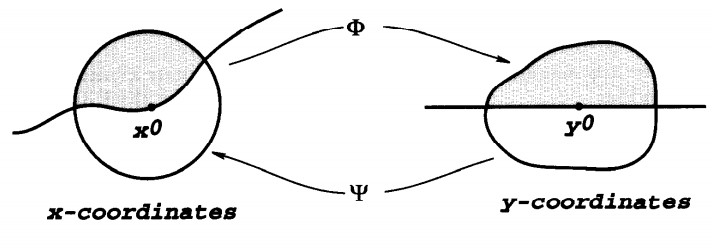
\includegraphics[scale=.5]{flatb}
\caption{Immagine da \cite[cap.8]{Evans}}
\end{figure}
\begin{remark}
Notiamo che $\Phi$ preserva l'eventuale analiticità della superficie $\Gamma^*$.
\end{remark}

Questa trasformazione ci fa capire come sia possibile scegliere di considerare  ``privilegiata''. Da qui in poi essa prenderà il nome di ``tempo'' e la indicheremo con la lettera $t$. Per essere più precisi rinominiamo le variabili nel modo seguente:
\begin{align*}
t & \leftarrow x_n \\
x & \leftarrow (x_1,\ldots , x_{n-1})
\end{align*}
Inoltre, introduciamo un po' di notazione che tornerà utile più avanti:
\begin{itemize}
\item chiamiamo $\Gamma_0 = \{t=0\}$.
\item indichiamo le derivate nel modo seguente: $D^\alpha_x D^j_t u$.
\end{itemize}
Concludiamo quindi che grazie alla trasformazione $\Phi$ otteniamo il nuovo problema:
\begin{equation}\label{gamma0prob}
\begin{cases}
F(x,t, D^\alpha_x D^j_t u)=0 & |\alpha | +j \leq k\\
D^j_t u (x,0)= \phi_j(x) & \text{per }j<k 
\end{cases}
\end{equation}
dove $u^*=u(\Phi)$.

\noindent\rule[0.5ex]{\linewidth}{0.2pt}

\begin{definition}
$\Gamma^*$ (o $\Gamma_0$) è non caratteristica se l'equazione su $\Gamma_0$ può essere riscritta in \textbf{forma normale} rispetto a $t$, ovvero se il problema \eqref{gamma0prob} può essere riscritto così:
\begin{equation*}
\begin{cases}
D_{t}^k u = G(x,t, D^\alpha_x D^j_t u) & |\alpha |+ j \leq k, \, j<k \\
D_t^ju = \phi_j & \text{ su } \Gamma_0, \, j<k
\end{cases} \\
\end{equation*}
\end{definition}

Per rendere più concreta questa definizione spesso si cercano delle condizioni sufficienti, ed eventualmente anche necessarie, perché l'equazione possa essere riscritta in forma normale, come abbiamo fatto noi nel paragrafo \ref{supcar} per i casi più semplici e come è stato fatto in \cite{Evans} e in \cite{Folland}.
Vediamo quindi di cosa si tratta, distinguendo i vari casi e ipotizzando di esserci già messi nella situazione \eqref{gamma0prob}:
\begin{itemize}
\item lineare e quasi-lineare: si richiede che $a_{(0,\ldots ,0,k)} \neq 0$ su $\Gamma_0$;
\item non lineare: si richiede la validità ipotesi teorema della funzione implicita (noto anche come teorema del Dini) su $F$, ovvero $D_{(D^k_t u)} F \neq 0$ su $\Gamma_0$.
\end{itemize}

\begin{remark}
Sempre rimanendo nell'ipotesi che la superficie sia $\Gamma_0$, a partire da queste considerazioni è facile vedere come la nuova definizione di superficie non caratteristica sia coerente con le definizioni del paragrafo \ref{supcar}.
\end{remark}

Ricordiamo, infine, che la nozione di superficie caratteristica ci deve garantire la possibilità di calcolare tutte le derivate parziali della soluzione sulla superficie. Per questa ragione l'impostazione di questa costruzione si ispira, in parte, a \cite[cap.3]{Evans}, dove è presente la dimostrazione di questa proprietà in due passi:
\begin{enumerate}
\item prima si ragiona ipotizzando di essere su $\Gamma_0$;
\item grazie alla trasformazione $\Phi$ si ottiene la proprietà per una generica $\Gamma^*$.
\end{enumerate}


\newpage
\section{Serie di potenze}
Dando per nota la teoria delle funzioni olomorfe, e di conseguenza anche la teoria base delle funzioni analitiche (reali), in questo paragrafo vogliamo scoprire, o conoscere meglio, solamente degli strumenti molto specifici che ci permetteranno di dimostrare il TCK.

Cominciamo con lo studiare uno sviluppo in serie di potenze di una funzione di cui non dobbiamo dimenticarci.
\begin{definition}
Funzione maggiorante: $$\mathcal{M}_{Cr}(x)=\frac{Cr}{r-(x_1+\ldots +x_n)}$$
\end{definition}
Utilizzando il teorema multinomiale, dimostriamo che la questa funzione può essere sviluppata in serie di potenze per $|x|<r/n$, ricavandone l'espressione dei coefficienti $c_\alpha$:
\begin{align*}
\mathcal{M}_{Cr}(x) &= \frac{Cr}{r-(x_1+\ldots +x_n)} = C \sum\limits_{j=0}^\infty \left(\frac{x_1+\ldots +x_n}{r}\right)^j  \\
&= C \sum\limits_{j=0}^\infty \frac{1}{r^j} \sum\limits_\alpha  \binom{|\alpha |}{\alpha } x^\alpha = \sum\limits_\alpha 
\underbrace{C \frac{|\alpha |!}{\alpha ! \, r^{|\alpha |}}}_{c_\alpha} \, x^\alpha .
\end{align*}

A partire da questo risultato, vogliamo enunciare due teoremi, che costituiscono la spina dorsale del cosiddetto metodo dei maggioranti, ideato per la prima volta da Cauchy, e che permettono di giustificare la terminologia introdotta poco fa.

\begin{theorem}[utilità del maggiorante]\label{teomagg}
\hpth{
g_\alpha \geq |f_\alpha|\\
\sum g_\alpha x^\alpha \text{ ha raggio di conv. } R
}{
\sum f_\alpha x^\alpha \text{ha raggio almeno } R
}
\end{theorem}


\begin{theorem}[costruzione del maggiorante]
\hpth{
\sum f_\alpha x^\alpha \text{ ha raggio } R
}{
\exists \, r<R, \, C>0 : \, |f_\alpha | \leq C \frac{|\alpha |!}{\alpha ! \, r^{|\alpha |}}
}
\end{theorem}

\begin{proof}
E' sufficiente notare che prendendo $C \geq |f_\alpha r^{|\alpha |}|$ si ha come conseguenza immediata che
$$|f_\alpha | \leq C \frac{1}{r^{|\alpha |}} \leq C \frac{|\alpha |!}{\alpha ! \, r^{|\alpha |}}.$$
\end{proof}

Nel caso in cui valgano le ipotesi del teorema \ref{teomagg} scriveremo:  $\sum g_\alpha x^\alpha \gg \sum f_\alpha x^\alpha$.

\begin{remark}
Gli stessi teoremi continuano a valere nel caso dei numeri complessi.
\end{remark}

Concludiamo il paragrafo e il capitolo con qualche proprietà per la manipolazione di serie di potenze. 
Prima di tutto occupiamoci dell'operazione di composizione.
\begin{theorem}
\hpthml{
y: \mathbb{R}^n \rightarrow \mathbb{R}^m \text{ tale che } y(x) = \sum y_\alpha (x-x_0)^\alpha \text{ in intorno di } x_0\\
g: \mathbb{R}^m \rightarrow \mathbb{R}^d \text{ tale che } g(y) = \sum g_\beta (y-y_0)^\beta \text{ in intorno di } y_0=y(x_0)\\
f = g \circ y
}{ 
\exists \; f_\gamma = P_\gamma (g_\beta, \, y_\alpha \text{ con } \alpha_i \leq \gamma_i) \text{ insieme di coeff. tali che } \\
- \; P_\gamma \text{ polinomi a coeff. non negativi }\\
-  \; f (x) = \sum f_\gamma (x-x_0)^\gamma
}
\end{theorem}
\begin{remark}
La forma dei polinomi $P_\gamma$ non dipende da $g$ e $y$.
\end{remark}
\begin{proof}
è facile convincersi di questo scrivendo esplicitamente la composizione delle due serie, specialmente per quanto riguarda il fatto che il coefficiente $f_\gamma$ dipenda solo dagli $y_\alpha$ tali che $\alpha_i \leq \gamma_i$.
\end{proof}

Ponendoci per semplicità nell'origine e recuperando la notazione $(x,t)$ del paragrafo precedente, enunciamo una semplice riscrittura di questo teorema.
\begin{theorem}[composizione]\label{composizione}
\hpthml{
y: \mathbb{R}^n \rightarrow \mathbb{R}^m \text{ tale che } y(x,t) = \sum y_{\alpha j} \; x^\alpha t^j \text{ in intorno dell'origine}\\
g: \mathbb{R}^m \rightarrow \mathbb{R}^d \text{ tale che } g(y) = \sum g_\beta \; y^\beta \text{ in intorno dell'origine }\\
f = g \circ y
}{
\exists \; f_{\gamma k} = P_{\gamma k} (g_\beta, \, y_{\alpha j} \text{ con } j \leq i) \text{ insieme di coeff. tali che } \\
- \; P_{\gamma k} \text{ polinomi a coeff. non negativi }\\
-  \; f (x,t) = \sum f_{\gamma k} \; x^\gamma t^k \label{seriepol} \numberthis
}
\end{theorem}

Un altro modo per ottenere una serie della tipologia in \eqref{seriepol} è sfruttare una derivazione rispetto a una qualsiasi variabile $x_i$. Vediamolo con il seguente teorema.
\begin{theorem}[derivazione]\label{derivata}
\hpth{
y: \mathbb{R}^d \rightarrow \mathbb{R}^m \text{ tale che } y(x,t) = \sum y_{\alpha j} \; x^\alpha t^j \text{ in intorno dell'origine}\\
}{
f=D_{x_i}y \text{ è una serie di potenze come in \eqref{seriepol} in intorno dell'origine}
}
\end{theorem}
\begin{proof} derivando termine a termine otteniamo
$$ D_{x_i} \sum y_{\alpha j} \; x^\alpha t^j = \sum  \underbrace{(\alpha_j+1) \, y_{(\alpha+e_i)j}}_{f_{\alpha j}} \; x^\alpha t^j. \; \footnotemark$$ \footnotetext{$e_i$ multi-indice vale 1 in corrispondenza della sua componente i-esima e 0 altrimenti}
E' immediato verificare le altre proprietà di $f_{\alpha j}$.
\end{proof}

Infine, siamo interessati a vedere cosa succede quando moltiplichiamo due serie come in \eqref{seriepol}, ottenute con uno dei metodi (teoremi \ref{composizione} e \ref{derivata}), a partire da una stessa serie $y$.
\begin{theorem}
\hpth{
f^1, f^2 \text{ serie costruite con uno dei due metodi a partire da una stessa } y
}{
f = f^1 f^2 \text{ è una serie di potenze come in \eqref{seriepol} in intorno dell'origine }
}
\end{theorem}

\begin{remark}
E' ammissibile anche il caso misto, in cui $f^1$ è ottenuta con una composizione e $f^2$ con una derivazione, e sarà proprio quello che utilizzeremo.
\end{remark}

\begin{proof} possiamo ricavare l'espressione dei coefficienti di $f$:
$$f_{\gamma k} = \sum_{\substack{\omega+\theta=\gamma \\ l+h=k}} f^1_{\omega l}\;  f^2_{\theta h}\, .$$
Di conseguenza $f_{\gamma k}$ sarà sicuramente un polinomio a coefficienti non negativi, poiché questa proprietà viene preservata da somme e prodotti. Inoltre, notando che $l,\, h \leq k$, si può mostrare che ogni singolo polinomio $f_{\gamma k}$ eredita la proprietà degli $f^1_{\omega l}$ e $f^2_{\theta h}$, vale a dire che esso dipende solo dagli $y_{\alpha j}$ dove $j \leq k$.
\end{proof}


\chapter{Il teorema di Cauchy-Kovalevski}
\section{Versione per EDO}
Versione per EDO
\section{Versione per EDP quasi-lineari}
IDEE CHIAVE: 

• RISCRIVERE L'EQUAZIONE IN FORMA DI EVOLUZIONE

• METODO DEI MAGGIORANTI: inserire nell'equazione delle serie di potenze, ottenere informazioni sui coefficienti, stimare questi coefficienti, dimostrare che la stima (una maggiorazione!) converge.

• METODO DELLE CARATTERISTICHE

Versione per EDP quasi-lineari
Rifacendoci a Evans, e quindi anche usando la notazione in esso presente, 
assumiamo che i coefficienti del sistema $B_j$ e $c$ abbiano come raggi di convergenza $r_{B_j}>0$ e $r_c>0$ 
di conseguenza per il Lemma nel capitolo 4.6.2 si osserva che affinché la maggiorazione valga è necessario 
che $r<\min\{\min_{j} \{r_{B_j}\}, r_c \}$.
Consideriamo ora la funzione $$\nu=\frac{r-s-\sqrt{(r-s)^2-2tCrmn}}{mn}$$ e ricordiamone alcune proprietà:
\begin{enumerate}[1.]

\item
E' interessante perché essa alla conclusione della dimostrazione del teorema di CK 
permette di scrivere in forma compatta la soluzione del problema maggiorante nella seguente forma: 
$$u = \nu(x_1+\ldots+x_{n-1}, t)[1,\ldots,1]^T$$

\item
Essa è analitica in un intorno dell'origine, in particolare per $t<\frac{(r-s)^2}{2Crmn}$ e di 
conseguenza anche in $B_h(0,0)$ con $h=\frac{r}{8Cmn}$.

\item
In $B_h(0,0)$ vale la condizione $s^2+m\nu ^2 (s,t)< r^2$

\item
Unendo le ultime due condizioni si ottiene che la soluzione è maggiorante in 

\end{enumerate}

\section{Versione per EDP non lineari}
Versione per EDP non lineari
Riscrivere l'equazione come un problema di evoluzione (vedi pdf)



\chapter{Esempi}

Dopo aver visto il TCK nella sua forma più nota, concentriamo ora lo sguardo su tre esempi importanti che aiutano a inquadrare meglio il ruolo che giocano le ipotesi e i limiti di questo teorema.

Tale discussione risulta particolarmente di rilievo, poiché per molto tempo si ritenne ragionevole pensare che un'equazione differenziale con coefficienti piuttosto regolari, come ad esempio $C^\infty$, dovesse avere almeno una soluzione. Questo, però, oltre al caso di analiticità trattato dal TCK, in generale non accade.


\section{Esempio di Lewy}
Questo primo esempio è decisamente il più importante ed interessante tra quelli qui trattati, 
proprio perché permette di introdurre in modo più rigoroso il problema appena citato.

Nel 1957 Hans Lewy propose questo semplice controesempio, volto a mostrare come l'ipotesi di \textbf{analiticità} nel teorema di 
Cauchy-Kowalevski fosse cruciale, portando un caso di un operatore differenziale lineare con coefficienti analitici che necessita 
della presenza di una forzante anch'essa analitica per possedere delle soluzioni almeno $C^1$.

\emergencystretch 3em
Ciò mostra come sia cruciale, non solo una discussione sulle condizioni sufficienti per l'esistenza di soluzioni locali, 
ma anche una sulle condizioni necessarie. Infatti Hörmander, matematico che contribuì ampiamente alla teoria delle equazioni lineari, 
rispose all'emersione di questo problema proprio con delle condizioni necessarie per l'esistenza di soluzioni locali 
(e quindi anche globali!) per equazioni lineari, le quali ispirarono poi a loro volta il lavoro di Treves e Nirenberg volto 
alla ricerca di condizioni necessarie e sufficienti.

\newpage
Preliminarmente si riportano qui sotto gli enunciati di due teoremi che torneranno utili nella discussione:

\begin{namedtheorem}[Formula di Green in $\mathbb{C}$]
\hpth{
D \subseteq \mathbb{C} \text{ dominio regolare }\\
f:D \rightarrow \mathbb{C}\\
f \in H(\interior{D})
}
{\oint\limits_{\partial^+D}f(z)\,dz=2i\iint\limits_D\frac{\partial f}{\partial \overline{z}}(x+iy)\,dxdy}
\end{namedtheorem}

\begin{remark}
La definizione di dominio regolare non ci tornerà particolarmente utile, infatti ai nostri scopi è sufficiente sapere che una qualsiasi palla chiusa è regolare (questo verrà utilizzato nella dimostrazione del teorema \ref{Lewy}). Per una formalizzazione di questo concetto si veda \cite[cap.8]{FMS}, dove è presente una trattazione dell'analogo teorema in $\mathbb{R}^2$ che va sotto il nome di ``Formule di Gauss-Green'' e ``Formula di Stokes'', di quale la generalizzazione in $\mathbb{C}$ è immediata.
\end{remark}

\begin{namedtheorem}[Principio di riflessione di Schwarz]
\hpth{
D \subseteq \mathbb{C} \text{ dominio regolare e simmetrico rispetto a } \mathbb{R}\\
D \cap\ \mathbb{R} \text{ è un intervallo }\\
f:D \rightarrow \mathbb{C}\\
f(\mathbb{R} \cap D) \subseteq \mathbb{R}\\
f \in H(\interior{D})
}
{f(\overline{z})=\overline{f(z)} \quad \forall z \in \interior{D}}
\end{namedtheorem}

\begin{remark}
La definizione di insieme simmetrico rispetto a $\mathbb{R}$ è data in modo naturale: esso deve soddisfare la condizione $z \in D \implies \overline{z} \in D$.
\end{remark}

Per entrare nel vivo dell'esempio, definiamo il seguente operatore:
$$L=D_x+iD_y-2i(x+iy)D_t$$
che ha dei coefficienti $C^\infty$ e il cui comportamento peculiare emerge dal teorema che enunciamo di seguito.

\begin{theorem}\label{Lewy}
\hpth{
f \text{ funzione continua a valori reali che dipende solo da } \; t\\
u\in C^1\;:\;Lu=f \text{ in un intorno dell'origine }
}
{f \text{ analitica in un intorno di } t=0}
\end{theorem}

\begin{proof}
Innanzitutto fissiamo un $R>0$ tale che $\{(x,y,t): x^2+y^2<R^2,|t|<R\}$ sia contenuto nell'intorno dell'origine delle ipotesi (ovviamente questo $R$ esiste sempre) e procediamo seguendo questi passi:
\begin{enumerate}[1.]
\item
Definiamo la funzione: 
\begin{equation*}
V(t,s)=\int\limits_{\gamma_r}u(x,y,t) \, dz \quad \text{con} \quad
\begin{system}
t \in (-R,R)\\
r^2=s \in [0,R^2)\\
\gamma_r=\partial^+B_r(0,0)\\
z=x+iy
\end{system}
\end{equation*}
\item
Troviamo una relazione tra $V_s$ e $V_t$:
\begin{align*}
V&=i\iint\limits_{B_r(0,0)}(u_x+iu_y)(x,y,t) \, dx \, dy &\text{per formula di Green}\\
&=i\int_0^r \int_0^{2\pi} (u_x+iu_y)(\rho \cos \theta,\, \rho \sin \theta,\, t) \, \rho \,d\rho \, d\theta &\text{in coordinate polari}\\
V_r&=i\int_0^{2\pi} (u_x+iu_y)(\rho \cos \theta,\, \rho \sin \theta,\, t) \, r \, d\theta &\text{derivando}\\
&=\int\limits_{\gamma_r}(u_x+iu_y)(x,y,t) \, r \, \frac{dz}{z}\\
V_s&=\frac{1}{2r}V_r=\int\limits_{\gamma_r}(u_x+iu_y)(x,y,t) \, \frac{dz}{2z}\\
&=\int\limits_{\gamma_r}u_t(x,y,t) \, dz + \int\limits_{\gamma_r}f(t) \, \frac{dz}{2z} &\text{usando } Lu=f\\
&=iV_t + \pi i f(t) \numberthis \label{eq:4}
\end{align*}
\item
Definiamo le funzioni:
\begin{align*}
F(t)&=\int_{0}^{t} f(\tau) \, d\tau\\
U(t,s)&=V(t,s)+\pi F(t)\;.
\end{align*}
e osserviamo le seguenti proprietà di $U$ vista come funzione di $w=t+is$: 
\begin{itemize}
\item
si può verificare che soddisfa l'equazione di Cauchy-Riemann $U_t+iU_s=2U_{\overline{z}}=0$ utilizzando la relazione \eqref{eq:4},
\item
è olomorfa per $(s,t) \in (0,R^2) \times (-R,R)$ per la proprietà precedente,
\item
è continua per $(s,t) \in [0,R^2) \times (-R,R)$ perché lo è $V$,
\item
$U(0,t)=\pi F(t)$ per $t\in (-R,R)$, ovvero assume valori reali sull'asse reale.
\end{itemize}
\item
Possiamo ora prolungare analiticamente $U$ in un intorno dell'origine, infatti, 
date le proprietà appena osservate, valgono le ipotesi del principio di riflessione di Schwarz che ci permette 
di definire $U$ per $s\in (-R^2,0)$ con la seguente formula: $$U(t,s)=\overline{U(t,-s)}.$$
\item
Concludiamo il ragionamento notando che, se il prolungamento di $U$ è analitico in un intorno dell'origine, lo deve essere anche $U(t,0)=\pi F(t)$ e anche $f=F'$.
\end{enumerate}
\end{proof}

\textbf{Generalizzazione.} Il teorema appena trattato si presta, in realtà, anche a una generalizzazione interessante e l'idea è la seguente: si cerca di mostrare che, nonostante la forma caratteristica di $L$ non abbia punti singolari, è possibile scegliere una forzante $F \in C^{\infty} (\mathbb{R}^3, \mathbb{R})$ in modo tale che \textbf{ovunque} l'equazione differenziale $Lu=F$ non ammetta soluzioni.

\begin{remark}
Dati due spazi matrici $(X,d_X)$ e $(Y,d_Y)$, con la notazione $C(X,Y)$ con $k \in \mathbb{N} \cup \{\infty\}$ indichiamo l'insieme delle funzioni continue del tipo $h:X \rightarrow Y$. Nel caso in cui $X=\mathbb{R}^n$ e $Y=\mathbb{R}^m$ useremo la notazione $C^k(\mathbb{R}^n,\mathbb{R}^m)$ naturalmente per le funzioni $C^k$.
\end{remark}

Prima di scendere nello specifico di questa seconda parte della discussione dell'esempio di Lewy, è utile richiamare tre definizioni:
\begin{definition}
Un sottoinsieme $D$ di uno spazio topologico $X$ è denso se per ogni $ A \in X$ aperto $D \cap A \neq \emptyset $.
\end{definition}
\begin{definition}
Un sottoinsieme $E$ di uno spazio metrico è senza parte interna se $\interior{E}=\emptyset$.
\end{definition}
\begin{definition}
Uno spazio topologico viene detto ``di Baire'' se l'unione numerabile di ogni famiglia di insiemi chiusi con interno vuoto ha interno vuoto.
\end{definition}

La ragione per cui sono stati citati questi concetti è che siamo interessati a un teorema, o per meglio dire, a un suo corollario, che permette di sviluppare un argomento per assurdo, nel caso si abbia a che fare con spazi metrici completi. Sono riportati di seguito gli enunciati.

\begin{namedtheorem}[Teorema della categoria di Baire]\label{Baire}
\hpthth{
(X,d) \text{ spazio metrico completo }\\
\{A_n\}_{n \in \mathbb{N}} \subseteq 2^X \text{ famiglia di insiemi aperti densi in } X\\
\{E_n\}_{n \in \mathbb{N}} \subseteq 2^X \text{ famiglia di insiemi chiusi e senza parte interna }
}
{\bigcap\limits_{n \in \mathbb{N}} A_n \text{ è denso in X }}
{\bigcup\limits_{n \in \mathbb{N}} E_n \text{ è senza parte interna }}
\end{namedtheorem}

\begin{remark}
Con questo teorema si mostra proprio come gli spazi metrici completi siano di Baire nella topologia indotta dalla metrica. Si veda \cite[cap.10]{RF} per la dimostrazione e maggiori dettagli.
\end{remark}

\begin{namedtheorem}[Corollario (argomento per assurdo di Baire)]\label{arg-Baire}
\hpth{
(X,d) \text{ spazio metrico completo }\\
\{E_n\}_{n \in \mathbb{N}} \subseteq 2^X \text{ famiglia di insiemi chiusi }\\
X=\bigcup\limits_{n \in \mathbb{N}} E_n
}
{\exists \, n \in N \text{ tale che } \interior{E_n} \neq \emptyset}
\end{namedtheorem}

\begin{remark}
Questo enunciato è la proposizione contronominale della Tesi 2 del teorema \ref{Baire} e, come abbiamo anticipato, può essere usato per ottenere un assurdo esibendo un spazio metrico completo uguale all'unione di una famiglia di insiemi chiusi e senza parte interna.
\end{remark}


Il secondo importante risultato di analisi funzionale, che giocherà un ruolo importante per raggiungere lo scopo dichiarato, è il teorema di Ascoli-Arzelà: un teorema ``di compattezza'', il quale sostituisce il teorema di Heine-Borel nel compito di ricerca di una sottosuccessione convergente, nel caso in cui non si abbia a che fare con spazi metrici di cui sia nota la proprietà di compattezza. In particolare, lo utilizzeremo per dimostrare che un insieme (di cui si capirà la struttura più avanti) è chiuso, sfruttando la proprietà di convergenza uniforme che la tesi garantisce.

Per comprendere a pieno l'enunciato di tale teorema, richiamiamo insieme ad esso due definizioni.
\begin{definition}
Una successione di funzioni $\{f_n:X\rightarrow\mathbb{R}\}_{n \in \mathbb{N}_0}$ si dice uniformemente limitata in $X$ se $\exists \, M\geq 0$ tale che $|f_n|\leq M$ in $X$.
\end{definition}
\begin{definition}
Una successione di funzioni $\{f_n:X\rightarrow\mathbb{R}\}_{n \in \mathbb{N}_0}$ si dice equicontinua in $X$ se $\forall \varepsilon >0 \;\, \exists \, \delta >0$ tale che $d(x,y)<\delta \implies \abs{f_n(x)-f_n(y)}<\varepsilon \quad \forall x,y \in X,\, \forall n \in \mathbb{N}_0 $.
\end{definition}
\begin{namedtheorem}[Teorema di Ascoli-Arzelà]
\hpth{
(X,d) \text{ spazio metrico completo }\\
\{f_n:X\rightarrow\mathbb{R}\}_{n \in \mathbb{N}_0} \text{ successione di funzioni }\\
\quad - \quad \text{uniformemente continua}\\
\quad - \quad \text{equilimitata}
}
{\exists \, f\in C(X,\mathbb{R}), n_k \text{ tali che } f_{n_k}\rightarrow f \text{ uniformemente }}
\end{namedtheorem}

Dopo aver inquadrato questi strumenti, è arrivato il momento di entrare nel merito della discussione e lo facciamo appoggiandoci a uno schema che presenta per punti e a grandi linee il ragionamento da affrontare:
\begin{enumerate}
\item
trasleremo il problema del teorema \ref{Lewy} in modo da ricondurci al caso di un generico punto $(x_0,y_0,t_0)$, usando come forzante la funzione $g(x,y,t)=f(t-2xy_0+2x_0y)$ (lemma \ref{lemma-tr});
\item
costruiremo una funzione $S_a \in C^\infty$ per ogni $a \in l^\infty$ (lemma \ref{lemma-serie});
\item
costruiremo degli insiemi $E_{j,n} \subseteq l^\infty$ chiusi e senza parte interna sfruttando $S_a$ e il teorema di Ascoli-Arzelà (lemma \ref{lemma-e});
\item
concluderemo la dimostrazione del teorema \ref{Lewy2} utilizzando i lemmi appena citati per ricavare, con un ragionamento per assurdo, l'uguaglianza $l^\infty = \bigcup E_{j,n}$, che ci permette di applicare l'argomento di Baire.
\end{enumerate}

Ora dettagliamo i passaggi appena elencati con enunciati e dimostrazioni.

\begin{lemma}\label{lemma-tr}
\hpth{
F \in C^\infty(\mathbb{R},\mathbb{R})\\
(x_0,y_0,t_0)\in \mathbb{R}^3\\
u\in C^1\;:\;Lu(x,y,t)=F'(t-2xy_0+2x_0y) \text{ in un intorno di } (x_0,y_0,t_0)\\
}
{F \text{ e } F' \text{ sono analitiche in un intorno di } t=t_0}
\end{lemma}

\begin{proof}
sfruttando l'invarianza dell'operatore $L$ rispetto a $$T(x,y,t)=(x+x_0,y+y_0,t+t_0+2xy_0-2x_0y),$$ ovvero la validità dell'identità (facile da verificare) $L(u \,\circ\, T)=(Lu) \circ T$, deduciamo che, se $u$ è soluzione dell'equazione delle ipotesi, essa rende vera in un intorno dell'origine anche l'espressione:
\begin{equation}\label{eq:10}
L(u \circ T)(x,y,t)=f(t+t_0) \text{ con } f=F'.
\end{equation}
Chiaramente $u \circ T \in C^1$ e $g(t)=f(t+t_0)$ soddisfano le ipotesi del teorema \ref{Lewy} e quindi applicandolo alla seconda equazione la tesi è dimostrata.
\end{proof}
\begin{remark}
L'analiticità di $F$ segue dall'ultimo passaggio della dimostrazione del teorema \ref{Lewy}, tendendo in considerazione del fatto che essa è della forma $F(t)=\int_{0}^{t} f(\tau)+c$ con $c\in \mathbb{R}$.
\end{remark}
\begin{remark}
L'equazione \eqref{eq:10} vale in un intorno dell'origine poiché l'operatore $T$ rende $\mathbb{R}^3$ un gruppo, noto in generale come gruppo di Heisenberg, e agisce in questo contesto come una traslazione.
\end{remark}

\begin{lemma} \label{lemma-serie}
\hpthth{
\{(x_j,y_j,t_j)\}_{j=1}^{\infty} \text{ denso in } \mathbb{R}^3\\ \label{eq:8} \numberthis 
c_j=2^{-j}e^{-\rho_j} \text{ con } \rho_j=|x_j|+|y_j| \quad \forall j \in \mathbb{N}_0\\
a=\{a_n\}_{n=1}^{\infty} \in l^{\infty}\\
F \in C^{\infty} (\mathbb{R},\mathbb{R}) \text{ periodica e non analitica }\\
f_j(x,y,t)=F'(t+2xy_j-2x_jy)
}
{S_a=\sum_{j=1}^{\infty} a_jc_jf_j \text{ converge uniformemente in } \mathbb{R}^3}
{\text{lo stesso vale per le derivate formali } D^{\alpha}S_a=\sum_{i=1}^{\infty} a_jc_jD^{\alpha}f_j}
\end{lemma}

\begin{remark}
Naturalmente $S_a$ è una funzione $C^\infty$.
\end{remark}

\begin{proof}
Siccome $F$ è $C^\infty$ ed è periodica definiamo $M_k=\sup_t\abs{F^{(k)}(t)} \in \mathbb{R} \quad \forall k \in \mathbb{N}\, .$
E ciò ci permette di scrivere, per ogni $\alpha$ multi-indice e $j\in \mathbb{N}_0$, le seguenti disuguaglianze:
\begin{align*}
|a_jc_jD^{\alpha}f_j| &\leq \norm{a}_\infty \, 2^{-j} \, e^{-\rho_j} \, M_{| \alpha |+1} \, \rho_j^{| \alpha |} \\
&\leq \norm{a}_\infty \, 2^{-j} \, M_{| \alpha |+1} \left(\frac{| \alpha |}{e}\right)^{| \alpha |}& \text{ poichè } \max\limits_{x \geq 0}\frac{x^{| \alpha |}}{e^x} = \left(\frac{| \alpha |}{e}\right)^{| \alpha |} \label{eq:5}\numberthis
\end{align*}
$D^\alpha S_a$ converge totalmente, e quindi anche uniformemente, essendo che la serie $$\sum_{j=1}^{\infty} \sup\limits_{\mathbb{R}^3} |a_jc_j D^{\alpha} f_j|$$ ha un termine generale minore o uguale della parte destra della disuguaglianza \eqref{eq:5}, la cui corrispondente serie numerica è ovviamente convergente.
\end{proof}

\begin{remark}
Prima di proseguire è soffermiamoci brevemente su due questioni:
\begin{itemize}
\item
$l^{\infty}$ è una spazio di Banach se dotato della norma: $\norm{b}_\infty=\sup_n|b_n|$ per ogni $b \in l^{\infty}$;
\item
esiste una funzione $f$ con le proprietà delle ipotesi: per esempio, la funzione $$F(x)=\sum_{n=1}^\infty\frac{\cos(n!\,x)}{(n!)^n}$$ è definita da un serie puntualmente convergente ed è $C^{\infty}(\mathbb{R},\mathbb{R})$, inoltre è periodica di periodo $2\pi$ e si può dimostrare che essa non è analitica in nessun punto $x\in\mathbb{R}$. Sopratutto per quest'ultimo aspetto si veda il problema 4 presente in \cite[cap.3]{John} per maggiori dettagli.
\end{itemize}
\end{remark}
\textbf{Notazione.} $A_{j,n} = B_{n^{-1/2}}(x_i,y_i,t_i)$ dove $(x_i,y_i,t_i)$ sono i punti nelle ipotesi del lemma \ref{lemma-serie}.
\begin{lemma}\label{lemma-e}
\hpth{
\text{Stesse ipotesi del lemma \ref{lemma-serie}}\\
\{E_{j,n}\}_{j,n \in \mathbb{N}_0} \subseteq l^{\infty} \text{ tali che } a \in E_{j,n} \; \iff \; \exists \, u \in C^1(A_{j,n}):\\
\quad - \quad Lu=S_a \text{ in } A_{j,n}\\
\quad - \quad u(x_j,y_j,t_j)=0 \numberthis \label{eq:9} \\
\quad - \quad |D^{\alpha}u| \leq n \text{ per } | \alpha | \leq 1 \text{ in } A_{j,n} \\
\quad - \quad |D^{\alpha}u(v) - D^{\alpha}u(w)| \leq n |v-w|^{1/n} \text{ per }
\begin{system}
| \alpha | = 1\\
v,w \in A_{j,n}
\end{system}
}
{\{E_{j,n}\} \text{ sono insiemi chiusi e senza parte interna}}
\end{lemma}

\begin{proof} 
dimostriamo separatamente separatamente le due proprietà:
\begin{enumerate}
\item
Per quanto riguarda la proprietà di chiusura, vogliamo mostrare che se $\{a^k\}\subseteq E_{j,n}$ è tale che $a^k \xrightarrow{l^\infty} a$ allora $a \in E_{j,n}$. Ciò, a sua volta, si riduce a mostrare l'esistenza di una funzione $u$ con le proprietà in \eqref{eq:9}.

Deduciamo immediatamente che $S_{a^k} \rightarrow S_a$ in modo uniforme, poiché $\abs{S_a - S_{a^k}} \leq M_1 \norm{a-a^k}$ per la \eqref{eq:5} con $\alpha = 0$. Inoltre, per le ipotesi su $a^k$ esiste una funzione $u_k$ che risolve l'equazione $Lu_k=S_{a^k}$ e che soddisfa le altre proprietà in \eqref{eq:9}. Proprio grazie a queste ultime $u_k$ soddisfa le ipotesi del teorema di Ascoli-Arzelà con $X=A_{j,n}$, quindi per una qualche $u$ vale che $u_{k_h} \rightarrow u \text{ uniformemente }$.

In particolare, sfruttando il fatto che $L$ è un operatore del primo ordine, si ricava facilmente che $Lu=S_a$ in $A_{j,n}$ poiché
\begin{align*}
Lu_{k_h}& \rightarrow Lu &\text{ uniformemente per le proprietà di } u_k\\
\lVert \quad &  &\\
S_{a^{k_h}}& \rightarrow S_a &\text{ uniformemente }
\end{align*}
e che $u$ eredita tutte le altre proprietà in \eqref{eq:9} da $u_k$ grazie alla convergenza uniforme.
 
\item
In ultimo si mostriamo che $\interior{E}_{j,n}=\emptyset$ ragionando per assurdo. Quindi, supponiamo che esista una successione $a$ interna a $\interior{E}_{j,n}$. Definendo poi
$$\delta_j = \frac{1}{c_j} \mathds{1}_{\{j\}} \in l^\infty,$$
osserviamo che esiste un $\theta \in \mathbb{R}$ abbastanza piccolo tale che $a'=a+\theta \delta_j \in E_{j,n}$.
Siano ora $u$ e $u'$ le soluzioni rispettivamente di $Lu=S_a$ e di $Lu=S_{a'}$ con le proprietà in \eqref{eq:9} e sia
$$u''=\frac{u'-u}{\theta}.$$ 
Chiaramente è vero che $u'' \in C^1$; inoltre, usando la linearità di $L$ e la definizione della serie $S$, è immediato vedere che vale la relazione $$Lu''=S_{\delta_j}=f_j,$$ ma ciò entra in contraddizione con il lemma \ref{lemma-tr} (di cui valgono tutte le ipotesi), non essendo $F$ analitica. 
\end{enumerate}
\end{proof}

\begin{theorem}\label{Lewy2}
\hpth{
A \subseteq \mathbb{R}^3 \text{ aperto }\\
}
{
\exists \, F \in C^{\infty}(\mathbb{R}^3,\mathbb{R}) \; : \; \nexists \, u \in C^1(A,\mathbb{R}) \text{ tale che }
\begin{system}
Lu=F \text{ in } A\\
u_x,\,u_y,\,u_t \text{ soddisfano} \\
\text {la condizione di Hölder }
\end{system}
}
\end{theorem}

\begin{remark}
L'arbitrarietà di $A$ implica che questo valga per tutti gli aperti di $\mathbb{R}^3$ e quindi che $Lu=F$ non abbia soluzioni $C^1$ e con derivate prime continue secondo Hölder da nessuna parte.
\end{remark}

\begin{remark}
La tesi implica come conseguenza naturale che non esistano nemmeno soluzioni $C^k$ per ogni $k \geq 1$, in quanto $C^k \subseteq C^1$.
\end{remark}

\begin{proof}
Ragionando per assurdo, concludiamo con i seguenti tre passi (di cui il secondo è quello che merita più attenzione).
\begin{enumerate}
\item
$E_{j,n} \subseteq l^{\infty} $ per ogni $j,n \in \mathbb{N}_0$ ovviamente.
\item
$a \in l^{\infty} \implies a \in E_{j,n}$ per qualche $j,n \in \mathbb{N}_0$ (i quali  dipendono da $a$).

Supponendo la tesi falsa, possiamo affermare che $\forall a \in l^\infty \; \exists \, A \in \mathbb{R}^3, \, u^* \in C^1(A,\mathbb{R})$ tali che si ha che $Lu^*=S_a$ e che $u^*$ ha le derivate prime continue secondo Hölder in $A$.

Si sa, inoltre, che per la densità dell'insieme dei punti in \eqref{eq:8} esiste un $(x_j,y_j,t_j) \in A$ ed essendo $A$ aperto esiste un $k$ (scelto abbastanza grande) tale per cui $A_{j,k} \subseteq A$.

Consideriamo ora la funzione $u=u^*-u^*(x_j,y_j,t_j)$, in modo che $u$ mantenga le proprietà di $u^*$, ma soddisfi al contempo la condizione $u(x_j,y_j,t_j)$ come richiesto in una della proprietà in \eqref{eq:9}.

In ultimo è chiaro che, essendo le derivate prime di $u$ continue secondo Hölder, esiste un $m$ abbastanza grande per cui valgono le condizioni rimanenti in \eqref{eq:9} con $m$ al posto del pedice $n$ e prendendo poi $n=\max\{k,m\}$ l'implicazione è dimostrata.

\item
Dai primi due passi concludiamo che $$l^{\infty}=\bigcup\limits_{j,n \in \mathbb{N}_0}E_{j,n},$$ ma, quindi, per il fatto che $l^{\infty}$ è di Banach e per le proprietà degli insiemi $E_{j,n}$, valgono sia le ipotesi del corollario \ref{arg-Baire} che la negazione della tesi. Ciò è assurdo.
\end{enumerate}
\end{proof}


\newpage
\section{Esempio di Kowalevski}

L'esempio su cui ci concentriamo ora è dovuto a Kowalevski stessa ed è stato utile a suo tempo a comprendere più a fondo, in modo quanto più essenziale possibile, l'importanza, o meglio la necessità, di assumere che la superficie scelta per assegnare i dati di Cauchy sia \textbf{non-caratteristica} per l'equazione differenziale in osservazione. Inoltre, costituisce un controesempio alla congettura proposta da Weierstrass, che suggeriva la possibilità di definire funzioni analitiche attraverso equazioni differenziali. 

Tutto ciò viene citato all'interno di una lettera rivolta a Fuchs (un matematico tedesco dell'Università di Berlino) scritta da Weierstrass (che supervisionò il lavoro di ricerca di  Kowalevski), con cui quest'ultimo faceva richiesta per l'accettazione delle tesi di dottorato di Sofya. La lettera è riportata integralmente in \cite[app.C]{Bio}.
 
Seguendo le orme di Kowaleski, consideriamo quindi il seguente problema di Cauchy per l'equazione del calore in una dimensione:
\begin{align}
\label{eq:1}
u_t-u_{xx}&=0\\ 
\label{eq:2}
u(x,0)&=\frac{1}{1+x^2} \quad \forall \, x \in \mathbb{R}
\end{align}
\begin{remark}
La condizione per $u_x$ su $\Gamma$ necessaria per completare il problema di Cauchy è già implicitamente imposta dall'equazione
\eqref{eq:2}.
\end{remark}
\begin{remark}
In realtà il dato iniziale realmente scelto da Kowalevski durante la sua ricerca è $\frac{1}{1-x}$, che però abbiamo deciso di non utilizzare qui per semplicità, evitando alcuni problemi legati alla singolarità della funzione e mantenendo invariato il significato del ragionamento.
\end{remark}
L'obiettivo che ci poniamo è quello di dimostrare che non ammette soluzioni analitiche in un intorno dell'origine.

\begin{enumerate}
\item
Per cominciare osserviamo che in questo caso la superficie su cui sono stati assegnati i dati di Cauchy $(1.2)$ è 
$\Gamma=\left\lbrace(x,t) \in \mathbb{R}^2:t=0\right\rbrace$. Essa in ogni punto ha come versore normale $(0,1)$ ed è, quindi,
caratteristica per l'equazione \eqref{eq:1}, poiché\footnote{vedi definizione \ref{supcarlin}}
$$\sum_{|\alpha|=2}^{\;} a_\alpha \boldsymbol{\nu}^\alpha = a_{(2,0)}\boldsymbol{\nu}^{(2,0)} = 0. $$
\item
Per assurdo supponiamo di avere una soluzione del problema $u$ analitica in un intorno dell'origine, ovvero:
$$u(x,t) = \sum_{\alpha = (\alpha_1, \alpha_2) }^{\;} c(\alpha) \, x^{\alpha_1} \, t ^{\alpha_2}, \quad
 c(\alpha) = \frac{D^\alpha u(0,0)}{\alpha!}$$
dove $|(x,t)|<r$ per qualche $r>0$.
\item
Calcoliamo i valori dei coefficienti $c(2n,0)$ $\forall n \in \mathbb{N}$.\\
Per fare questo dobbiamo sviluppare in serie di potenze centrata nell'origine la funzione del problema di Cauchy:
$$\frac{1}{1+x^2} = \frac{d}{dx}\arctan(x) = \frac{d}{dx}\sum_{n=0}^{\infty}\frac{(-1)^n}{2n+1} \, x^{2n+1} 
= \sum_{n=0}^{\infty}(-1)^n \, x^{2n} \quad \forall x \in \mathbb{R}.$$
Da questa serie otteniamo le relazioni:
\begin{align*}
D_x^{2n}u(0,0) &= \frac{d^{2n}}{dx^{2n}} \left. \frac{1}{1+x^2}\right|_{x=0} = (-1)^n (2n)!\\
D_x^{2n+1}u(0,0) &= \frac{d^{2n+1}}{dx^{2n+1}} \left. \frac{1}{1+x^2} \right|_{x=0} = 0
\end{align*} 
Dalle quali si ricava: $c(2n,0)=(-1)^n$ e $c(2n+1,0)=0$.
\item
Calcoliamo i valori dei coefficienti $c(2n,n)$ e dimostriamo che  $c(2n,n) \xrightarrow{n\rightarrow\infty} +\infty$.\\
A questo scopo, invece, si sfruttiamo l'equazione \eqref{eq:1} per ottenere la seguente relazione tra i coefficienti:
\begin{equation} 
\label{eq:3}
c(\alpha_1,\alpha_2+1) = \frac{(\alpha_1+2)(\alpha_1+1)}{(\alpha_2+1)} \, c(\alpha_1+2,\alpha_2).
\end{equation}
E utilizziamo, quindi, quest'ultima come segue:
\begin{align*}
c(2n,n) &= \frac{(2n+2)(2n+1)}{n} \, c(2n+2,n-1)   &\eqref{eq:3}\quad\text{con} \quad 
\begin{system}
\alpha_1=2n\\
\alpha_2+1=n
\end{system}\\
 &= \ldots = \frac{(2n+2n)\cdots(2n+1)}{n!} \, c(2n+2n,0) &\text{\quad iterando su } n\\
 &= \frac{(4n)!}{(2n)! \, n!} (-1)^{2n} \\
 &\sim \frac{1}{\sqrt{\pi n}}\left(\frac{64n}{e}\right)^n \xrightarrow{n\rightarrow\infty} +\infty  &\text{per la formula di Stirling}
\end{align*}
\item
Completiamo il ragionamento in modo immediato osservando che 
$$c(2n,n) \, x^{2n} \, t ^{n}\xrightarrow{n\rightarrow\infty} +\infty \quad \forall (x,t) \neq (0,0),$$ 
infatti ciò implica direttamente che la serie di potenze non converge in ogni punto diverso dall'origine e questo è assurdo.
\end{enumerate}

\newpage
\section{Esempio di Hadamard}
L'ultimo esempio che affrontiamo, dovuto ad Hadamard (1932), aiuta a capire un limite importante del TCK, ovvero il fatto che esso non fornisca alcun controllo sulla \textbf{relazione} tra i dati di Cauchy e la forma della soluzione analitica, la quale potrebbe risultare instabile. 

Per osservare tale comportamento consideriamo il seguente problema di Cauchy per l'equazione di Laplace in due dimensioni al variare di $n$:
\begin{align*}
u_{xx}+u_{yy}&=0\\
u(x,0)&=0 \numberthis \label{eq:6}\\ 
u_y(x,0)&=n\sin(nx)e^{-\sqrt{n}} \quad \text{con} \quad n\in\mathbb{N}
\end{align*}


Quello che vogliamo mostrare è come al crescere di $n$ si verifica un blow-up della soluzione $u_n$ del problema \eqref{eq:6}.
\begin{enumerate}[1.]
\item
Il problema, come nell'esempio precedente, è assegnato su $\Gamma=\left\lbrace(x,y) \in \mathbb{R}^2:y=0\right\rbrace$, che è naturalmente una superficie non caratteristica per l'equazione di Laplace (si noti infatti che essa è ellittica e quindi non possiede alcuna superficie caratteristica).
\item
E' facile verificare che la funzione $u_n(x,y)=\sin(nx)\sinh(ny)e^{-\sqrt{n}}$ soddisfa \eqref{eq:6} e che essa è analitica, per questo è anche l'unica possibile con quest'ultima proprietà.
\item
Si osserva, infine, come $\sinh(ny)e^{-\sqrt{n}}\xrightarrow{n\rightarrow\infty} \infty$.
\end{enumerate}
Come conclusione di questa discussione è interessante osservare anche come la soluzione non dipenda con continuità dai dati. 
Infatti, considerando il problema per ${n=\infty}$, ovvero con dati $u(x,0)=u_y(x,0)=0$, notiamo immediatamente che l'unica soluzione analitica è $u\equiv0$, la quale è profondamente diversa dal comportamento asintotico di $u_n$.

A partire da queste considerazioni Hadamard proseguì i suoi studi, prima definendo il concetto di buona positura di un problema di Cauchy\footnote{un problema di Cauchy è ben posto se ha una e una sola soluzione stabile rispetto ai dati}, e poi scoprendo che i problemi costruiti con equazioni iperboliche a coefficienti costanti soddisfano sempre questa nella classe delle funzioni $C^\infty$.


\chapter{Versioni alternative}
(classica e astratta)

Ispirazione a Ovsyannikov, L.V. (vedi bibliografia) (vedi pag 109 e 110 treves analytic)

classi di Ovsyannikov
\chapter{Conseguenze}
\section{Teorema di Holmgren}

\section{Altre applicazioni}
teorema inutile nella pratica che però ha ispirato ricerche e scoperte future cruciali e utili (come accadde per i grafi di eulero)

applicazioni:
\begin{itemize}
\item fisica matematica (cosa succcede nella realtà quando si hanno soluzioni analitiche locali?)
\item teorema di holmgren
\item teorema di cartan-kahler (pag 137) utile in geometria differenziale (suggerisce Tao), economic theory (microeconomia, ekeland e chiappori, 1999) per l'eistenza locale di una funzione utilità concava (e quindi con un massimo) ricavata da un sistema di pdes che neccessita di dati analitici (visto come un sistema differenziale esterno)
\end{itemize}

I. Ekeland

Cartan Kahler

4 (with Chiappori), "Aggregation and market demand: an exterior differential calculus viewpoint", Econometrica, 67 (1999), p. 1435-1458

This paper solves a basic problem in economic theory, which had remained open for thirty years, namely the characterization of market demand functions. The method of proof consists of reducing the problem to a system of nonlinear PDEs, for which convex solutions are sought. This is rewritten as an exterior differential system, and is solved by the Cartan-Kähler theorem, together with some algebraic manipulations to achieve convexity. The introduction of exterior differential calculus proved to be a breakthrough, and was the starting point of a long collaboration with P.A. Chiappori. We realized that the mathematical structure we had discovered in this problem was to be found also in one of the major problems of econometrics: given a group (a household, for instance), can one characterize and identify the preferences of each member if one observes only the collective demand ?. I am happy to say that this research program is now concluded, with the publication of two major papers [14] and [25] and a100-pages survey [28] which will probably turn into a book.

14: (with P.A. Chiappori) "The microeconomics of group behaviour: general characterization". Journal of Economic Theory, september 2006 , volume 130 (p.1 – 26)

25: (with P.A. Chiappori) "The microeconomics of group behaviour: Identification". Econometrica, 2005, 44 pages

28: (with P.A. Chiappori). "The mathematics and economics of aggregation". Foundations and Trends in Economic Theory, 2009

% BIBLIOGRAFIA
% PER FARLA FUNZIONARE: eseguire latex-bibtex-latex-latex
\addcontentsline{toc}{chapter}{Bibliografia}
\nocite{*} % Inserire nella bibliografia anche le fonti non citate esplicitamente nel testo
\bibliographystyle{alpha} % We choose the "plain" reference style
\bibliography{bibliografia} % Entries are in the refs.bib file

\end{document}